%% !TeX root = report.tex

Transformata Burrowsa-Wheelera nie jest metodą kompresji, a jedynie
sposobem modyfikacji danych (położenia poszczególnych bajtów). Po
modyfikacji dane wyjściowe zawierają zazwyczaj ciągi równych sobie
bajtów umieszczonych po sobie. Tak ułożone dane lepiej poddają się
kompresji. Algorytm transformaty Burrowsa-Wheelera zaimplementowano
zgodnie z opisem w \cite{kompresja}.

Strumień danych wejściowych dzielony jest na bloki o rozmiarze będącym
parametrem algorytmu. Dane w każdym bloku sortowane są metodą sortowania
przedrostków (ang. \emph{Suffix Sorting}) - opis algorytmu sortowania
znajduje się w kolejny akapicie. Wynikiem sortowania jest macierz
indeksów sortowanych bajtów. Dane wyjściowe tworzone są poprzez przeglądanie
posortowanej macierzy indeksów - jako wynik zastosowania transformaty
należy zwrócić dane skonstruowane poprzez kolejne wypisywanie bajtów
z pozycji \emph{i-1}, gdzie \emph{i} jest wartością zapisaną w macierzy
indeksów. Dla \emph{i=0} należy wypisać ostatni bajt z bloku. Do tak
wypisanych danych należy dołączyć liczbę wskazującą pozycję na której
znalazł się bajt o indeksie 1 z bloku wejściowego.

W implementacji Transformaty Burrowsa-Wheelera najbardziej problematycznym
krokiem algorytmu jest sortowanie bajtów metodą sortowania przedrostków.
Krok ten jest problematyczny ze względu na swoją złożoność czasową.
Algorytm sortowania spowodował również najwięcej problemów podczas
implementacji transformaty. W projekcie po dokonaniu przeglądów algorytmów
sortowania przedrostkowego zdecydowano się zaimplementować algorytm
Itoh'a (wg opisu w {[}2{]} (thesis.ps)).\\
 Algorytm sortowania składa się z 3 kroków: 
\begin{enumerate}
\item W pierwszym kroku należy podzielić dane na dwa typy: X i Y. Wykonujemy
to przeglądając bajty w bloku i jeśli obecnie analizowany bajt jest
leksykograficznie po następnym bajcie, wtedy zaznaczamy go jako należący
do X. W przeciwnym przypadku jest on typu Y. Ostatni bajt z bloku
należy porównywać z pierwszym bajtem tego samego bloku. (Rys. \ref{fig:Podzia=000142-danych-wej=00015Bciowych})
\item W drugim kroku sortujemy dane przez zliczanie, umieszczając w tablicy
najpierw dane typu X, a później typu Y. Dane typu Y sortujemy zmodyfikowanym
algorytmem Radix Sort, jeśli dla danego symbolu jest więcej elementów
typu Y, niż 1. Modyfikacja algorytmu Radix Sort polega na tym, iż
rozpoczyna on analizowanie danych od najbardziej znaczących bajtów,
a nie tak jak w swej standardowej wersji - on najmniej znaczących.
Dzięki temu poza przypadkami długich ciągów takich samych bajtów nie
ma potrzeby analizowania całego bloku dla każdego sortowanego bajtu.
Algorytm zaimplementowano iteracyjnie - z użyciem stosu umieszczonego
na stercie. 
\item W trzecim kroku następuje łączenie koszyków w następujący sposób -
przeglądamy częściowo posortowany blok wejściowy (posortowane są tylko
dane typu Y). Jeśli dla \emph{i} będącego pozycją elementu z posortowanego
bloku w pierwotnym bloku (wejściowym), bajt na pozycji \emph{i-1}
jest typu X, to należy go umieścić na pozycji, na której powinien
się znajdować ze względu na swoją wartość i przesunąć wskaźnik dla
tej wartości. 
\end{enumerate}
\begin{wrapfigure}{o}{0.5\columnwidth}%
\centering
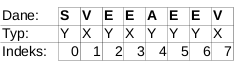
\includegraphics{\PICSDIR/bwt_dane}

\caption{\label{fig:Podzia=000142-danych-wej=00015Bciowych}Przykład - podział
danych wejściowych na typy}
\end{wrapfigure}%
%

\begin{figure}
\centering
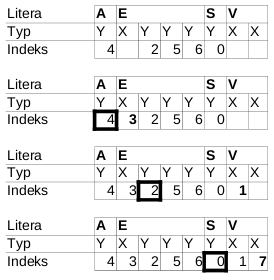
\includegraphics{\PICSDIR/bwt_dane3}

\caption{\label{fig:Spos=0000F3b-wstawiania-bajt=0000F3w}Przykład - sposób
wstawiania bajtów typu X do posortowanej tablicy. W pogrubionej ramce
znajduje się element powodujący wstawienie pogrubionego elementu typu
X.}

\end{figure}
Niewątpliwą zaletą zastosowanego algorytmu jest fakt, iż występujące
w kroku 3 łączenie koszyków ma złożoność liniową, co oznacza, że bajty
z koszyka X zostały posortowane w czasie liniowym. Pewną wadą przyjętego
rozwiązania jest to, iż w zależności od charakteru danych, spora ich
część trafia do koszyka Y, który jest już sortowany algorytmem Radix
Sort - podatnym na głęboką rekurencję.

Podczas dekodowania danych (transformata odwrotna - przywracająca
pierwotne ułożenie bajtów w bloku) stosowane jest sortowanie przez
zliczanie - ponieważ podczas dekodowania wystarczy posortować bajty
leksykograficznie (ściślej: tworzona jest tablica indeksów wskazujących
na posortowane dane). W związku z tym dekodowanie danych jest dużo
szybsze, niż kodowanie - algorytm sortowania przez zliczanie ma złożoność
liniową w stosunku do długości bloku. Pozostałe działania wykonywane
podczas dekodowania również posiadają liniową złożoność.

W transformacie bardzo ważny jest algorytm sortowania, ponieważ błędne
posortowanie danych powoduje przekłamania w odkodowanych danych.
